\chapter{Background}
\label{chap:background}


\section{Mathematical logic}

\todo{Javítani a többi sectiont ez alapján}

Mathematical logic is useful for deciding correctness of systems. This section provides some insight about propositional logic, first order logic, and the satisfiability problem. Differenece logic is also introduced.

\subsection{Propositional logic}

Propositional logic (or zeroth order logic) is concerned with the study of formulae of boolean variables, and deciding whether they are true or false. Propositional formulae are composed of truth symbols $\top$ (true) and $\bot$ (flase),  and propositional variables $p,q, \dots$ with the use of logical connectives. A formula $\varphi$ can be an atom (a truth symbol or a variable) or can be constructed from other logical formulae with the following connectives:

\begin{itemize}
	\item negation: $\neg\varphi$ is evaluated true iff $\varphi$ is evaluated false (formal equivalent of 'not'),
	\item conjunction: $\varphi_1 \wedge \varphi_2$ is evaluated true iff  both $\varphi_1$ and $\varphi_2$ is evaluated true (formal equivalent of 'and'),
	\item disjunction: $\varphi_1 \vee \varphi_2$ is evaluated true iff  at least one of $\varphi_1$ and $\varphi_2$ is evaluated true (formal equivalent of 'or'),
	\item implication: $\varphi_1 \to \varphi_2$ is evaluated true iff  $\varphi_1$ is evaluated false or both $\varphi_1$ and $\varphi_2$ is evaluated true (formal equivalent of 'if \ldots then'),
	\item equivalence: $\varphi_1 \leftrightarrow \varphi_2$ is evaluated true iff   both $\varphi_1$ and $\varphi_2$ is evaluated true or  both $\varphi_1$ and $\varphi_2$ is evaluated false (formal equivalent of 'if and only if').
\end{itemize}

\emph{Note:} disjunction, implication, and equivalence can be expressed using negation and conjunction. These operators are only defined to raise the level of descriptive power.

The (boolean) satisfiability problem (SAT, for short) can be defined as follows.
\begin{description}
	\item[Input]: A propositional logic formula $\varphi$.
	\item[Output]: \emph{Yes} if $\varphi$ is satisfiable (i.e. it is possible to ground the variables appearing in $\varphi$ to truth symbols so that $\varphi$ is evaluated true), \emph{No} if not.
\end{description}

\subsection{First order logic}

Propositional logic is useful, however, sometimes its expressive power is not enough. First order logic is a extends propositional logic with predicates, functions and the quantifiers $\exists$ (existential quantifier) and $\forall$ (universal quantifier). While propositional logic formulae could only be evaluated to truth values, first order logic formulae can be evaluated to numbers, or any abstract concept.

The basic elements of first order logic are \emph{terms}. Variables and constants (0-ary functions) are terms, as well as $n$-ary functions applied $n$ terms. In first order logic an atom can be $\top, \bot$ or an a $n$-ary predicate applied to $n$ terms. Formuale are gained by applying connectives (the same as in case of propositional logic) and quantifiers to atoms.

The satisfiability problem can be applied to first order logic formulae, but it is undecidable. However, there is a variant of the problem that is applicable, and solveable for most practical problems. The key idea is to formalize strucures.

\begin{dfn}
	A \emph{first order theory} $\mathcal{T}$ is a pair $(\Sigma,\mathcal{A})$  where
	\begin{itemize}
		\item $\Sigma$ is the \emph{signature}, i.e. the set of constant, function and predicate symbols and
		\item $\mathcal{A}$ is the set of \emph{axioms} where an axiom is a first order logic formula that has no quantifiers in it, and $\Sigma$ contains all constants, functions and predicates appearing in it.
	\end{itemize}
\end{dfn}

The \emph{Satisfiable Modulo Theories} (SMT) for short can be defined as follows.
\begin{description}
	\item[Input]: A theory $\mathcal{T}=(\Sigma,\mathcal{A})$, and $\Sigma$-formula $\varphi$.
	\item[Output]: \emph{Yes} if $\varphi$ is satisfiable in $\mathcal{T}$, \emph{No} if not.
\end{description}

In many practical theories, SMT becomes solveable.

\subsection{Difference logic}

An atom in (integer) difference logic is a logical expression of the form $x-y<n$ or $x-y \leq n$ where $x$ and $y$ are variables defined over $\mathds{Z}$ and $n$ is a constant. A difference logic formula $\varphi$ is a conjunction of one ore more atoms. In case of difference logic, SAT is not only decidable, but polynomial.

Since framework presented in this paper relies on a SAT (SMT) solver (as it is explained in chapter \ref{chap:impl}), this paper does not adress the algorithms for deciding satisfiability (if it is decidable). For more information on satosfiability, the reader is referred to \todo{hivatkozás}.


\section{Formal verification}

Formal verification is the act of proving the correctness or incorrectness of a system in a mathematically precise way. Model checking is an automatic formal verification technique,where the system has to be represented by a formal model, and the requirements of the system has to be a property of the system formally defined as logical formulae. Verification can be performed by proving that the system (represented by the formal model) satisfies that property.

\subsection{Modeling formalisms}
It is important to find the appropriate representation of the model i.e. the appropriate formalism in order to be able to model and check the property. This paper focuses on \emph{behavior properties} examined on \emph{behavioral models}.

\subsubsection{Finite automata}

The finite automaton (plural: automata)  is one of the most common formalisms for modeling behavior. This way the system is described by a finite set of possible states, and a set of steps defining the system's state changes.

\begin{dfn}
	Formally a \emph{finite automaton}, or state machine $\mathcal{A}$ is a touple $\langle S,s_0,T \rangle$ where
	\begin{itemize}
		\item $S$ is a finite set of states,
		\item $s_0 \in S$ is the initial state and
		\item $T \subseteq (S \times S)$ is a set of transitions.
	\end{itemize}
\end{dfn} 

Structurally $\mathcal{A}$ can be represented as a directed graph $G_\mathcal{A}$ where $V(G_\mathcal{A})=S$ and $E(G_\mathcal{A}})=T$. The system's operation is described as follows.

Initially, the system is in $s_0$. The system can change its state to some other state $s_1$ iff $(s_0,s_1) \in T$. from $s_1$ it can change its state to $s_2$ iff $(s_1,s_2) \in T$, and so on. 

\begin{example}
	\todo{példa}
\end{example}

This formalism is easy to use and verify, but its expressive power is not necessary: there are many types of behavoiurs that can't be modelled this way.

\subsubsection{Finite automaton extended with variables}

Many extensions of the finite automaton are known with various levels of expressive power. The following extension lifts the level of expressive power to that of Turing-machines: extending the automaton with variables.



A finite automaton extended by variables could be (briefly) defined as a touple $\langle L,l_0,v_0, E, I\rangle$ operationg on a set of variables $\mathcal{V}$ where
\begin{itemize}
	\item $L$ is the set of control locations,
	\item $l_0 \in L$ is the initial location,
	\item $v_0$ is a function assigning an initial value to each variable $x \in \mathcal{V}$,
	\item $E \subseteq L \times \mathcal{B} \times \mathcal{U} \times L$ is the set of edges (where $\mathcal{B}$ can be briefly described as the set of bool valued first oreder logic formulae constructed from the variables of $\mathcal{V}$,  and $\mathcal{U}$ can briefly defined as the set of unary functions operating on subesets of $\mathcal{V}$  assigning new values to variables) and
	\item $I: L \to \mathcal{B}$ assigns invariants to locations.
\end{itemize}

Instead of states, the graph's nodes are called control locations, since the system's state also depends on the values of the variables. For similar reasons, the edges of the graph are now called edges in the formalism aswell, and they are more expressive: an edge $e=(l,g,a,l')$ represents a transition form $l$ to $l'$, with a guard $g$ and an assignment function $a$. A guard is a condition that has to be satisfied in order for the transition to be enabled. The function $a$ describes how the value of some variables is changed during the transition. Locations can have invariants, that are conditions that have to be satisfied while the system stays in that location.

The system's operation starts from the control location $l_0$, and the variables are intialized as $v_0$ defines. A system can transition from $l$ to some $l'$ if there exist an edge $e=(l,g,a,l')$ where $g$ is satisfied by the variables current values, and $I(l')$ is satisfied by the values $a$ assigns to the variables (or their current value if $a$ is undefined on them).

\begin{example}
	\todo{példa - előző kiegészítve}
\end{example}

\subsection{Reachability}
During formal verification, one of the most important questions is reachability: deciding whether a system can step into a given state. In many cases, the state in question represents an erroneous state and the desired outcome of model checking is that it is unreachable.

The problem can be defined as follows.
\begin{description}
	\item[Input]: A system $S$ and a state $s_{err}$.
	\item[Output]: \emph{Yes} if it is possible for $S$ to operate in a way that it eventually steps in $s_{err}$, \emph{No} if not.
\end{description}

When the answer is \emph{Yes}, it is useful to provide a \emph{counterexample}: an execution trace $\sigma = s_0 \to s_1 \to \cdots \to s_{err}$ setting the systems's state to $s_{err}$ where $s_i$-s are states  and $s_i \to s_{i+1}$ notations represent possible steps of the system from $s_i$ to $s_{i+1}$.

Each formalisms have their own interpretation of the problem - regarding how erroneous states and execution traces are described. For example, in case of finite automata, the problem can be interpreted as follows. 

\begin{description}
	\item[Input]: A finite automaton $\mathcal{A}=\langleS,s_0,T\rangle$ and a state $s_{err} \in S$.
	\item[Output]: A sequence of states and transitions $\sigma = s_0 \xrightarrow{t_0} s_1 \xrightarrow{t_1} \cdots \xrightarrow{t_n} s_{n+1}=s_{err}$ ($s_i \in S, t_i=(s_i,s_{i+1}) \in T$ for all $0 \geq i \geq n$) if the $\mathcal{A}$ can reach $s_{err}$ , \emph{No} if not.
\end{description}

This problem can be solved by any pathfinding algorithm executed on $G_\mathcal{A}$.

\begin{example}
	\todo{valami egyszerű példa megoldással}
\end{example}

In case of extended finite automata the problem can be interpreted as follows.
\begin{description}
	\item[Input]: A finite automaton $\mathcal{A}=\langle L,l_0,v_0, E, I\rangle$ and a control location $l_{err} \in L$.
	\item[Output]: A sequence of locations and enabled transitions $\sigma = l_0 \xrightarrow{e_0} l_1 \xrightarrow{e_1} \cdots \xrightarrow{e_n} l_{n+1}=l_{err}$ if the $S$ can reach $s_{err}$, \emph{No} if not.
\end{description}

Note, that in this case error states are defined solely by the location, however, it is easy to reduce a problem where the values of the variables are also constrained into this form.

\begin{example}
	\todo{példa?}
\end{example}

The described problem is unsolveable as well as the reachability problem for all other Turing-complete formalisms. This is one of the reasons why the modeling formalism has to be chosen carefully. A 'simple' formalism may not have enough expressive power to percisely model the system, while verification of more complex formalisms may be ineffective or even impossible.

\subsubsection{Statespace exploration}

Even if reachability is undecidable (or just ineffective), there are many methods and approaches on how to gain useful information on the problem. The most obvious approach is \emph{statespace exploration}.

\begin{dfn}
	The \emph{statespace} of a system is the set of states that are reachable from the initial state by a sequence of enabled transitions. 
\end{dfn}

The idea of statespace exploration is to systematically list all possible states in the statespace. If the erroneous state is found the system is proven to be incorrect. Otherwise if all possible states are listed (in case of a finite statespace) and no erroneous state is found, the system is proven to be correct. (In case of an infinite statespace this process may never terminate.)

One of the simplest ways for exploring the statespace is by constructing a search-tree. The root of the tree is the initial state $s_0$ of the system. The statespace is explored by iteratively chosing a leaf with a state $s$ of the tree, and introducing a new edge for all possible enabled transitions $(s,s')$ pointing to a new node with a state $s'$. This way, all possible execution traces are explored, but states may appear more than once if there are more execution traces to reach them.

It is also possible to construct a state graph, where the statespace is explored similarly, except one state can only appear on one node. This helps reducing the size of the graph, however (in case of an infinite statespace) it still might be infinite. Infinite statspaces can never be completely explored this way (by explicit exploration), however, sometimes, when small counterexamples are expected, it is not necessary.

Consider the \emph{bounded reachability problem}.
\begin{description}
	\item[Input]: A system $S$, a state $s_{err}$, and a bound $k$.
	\item[Output]: A counterexample, if $S$ can reach $s_{err}$ in at most $k$ steps, \emph{No} if not.
\end{description}

This problem is decidable, even for finite automata with variables. Even so, explicit statespace exploration can not be considered an effective method.

\subsection{CEGAR}

One of the possible approaches to perform more effective model checking is abstraction. A less detailed system model is constructed that hides unimportant parts of the behavior providing a model of complex statespace overapproximating the original one. The idea of counterexample guided abstraction refinement (CEGAR) \cite{clarke2003counterexample} is to apply 
model checking to this simpler model, and then examine the results on the original one. The idea is illustrated on
Figure \ref{fig:cegar}.


\begin{figure}
	\centering
	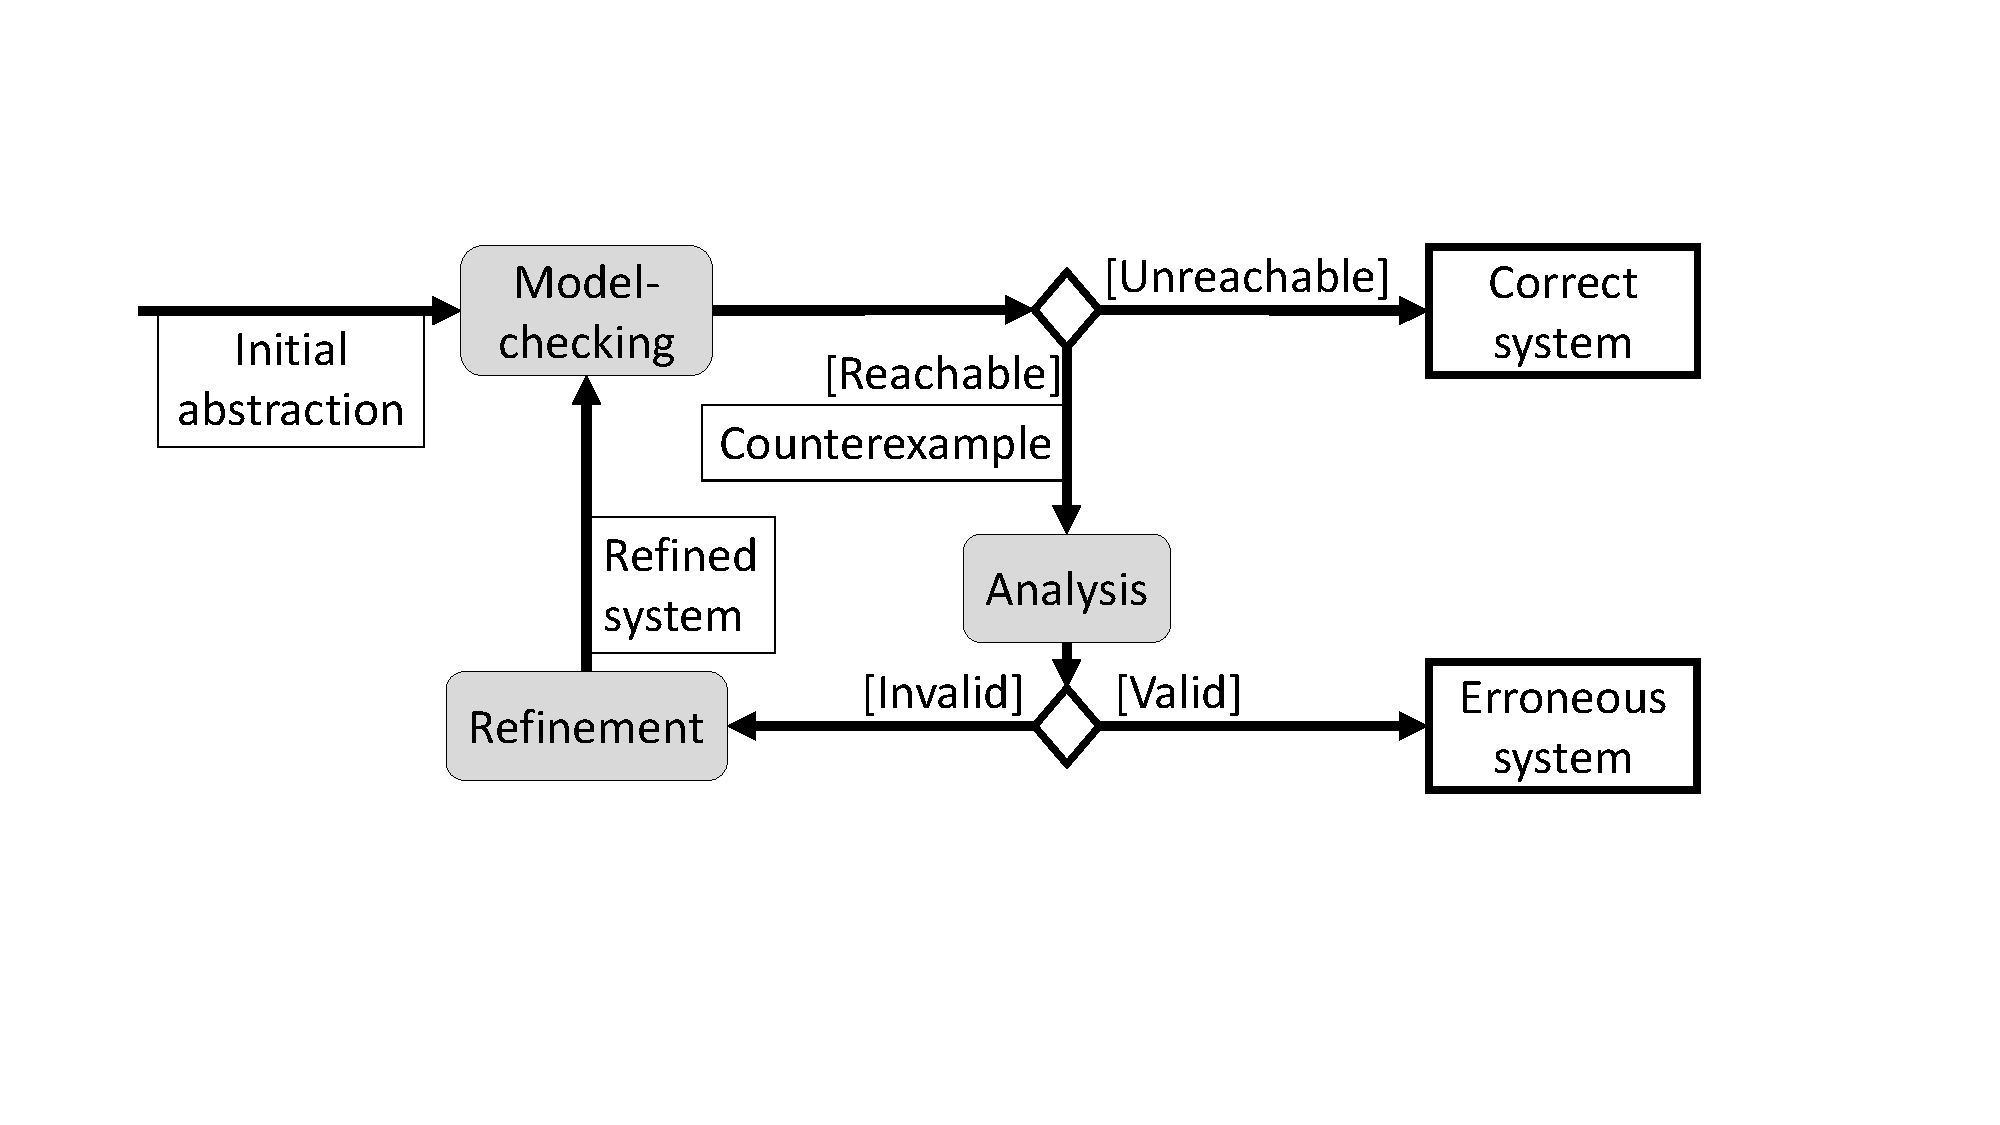
\includegraphics [width=0.7\textwidth] {include/figures/cegar_flow_black}
	\caption{Counterexample-guided abstraction refinement}
	\label{fig:cegar}
\end{figure}

%The CEGAR approach introduced in \cite{clarke2003counterexample} makes
%abstraction refinement a key part of model checking. 

First, an abstract system is constructed. The key property of abstraction is
that the state space of the abstract system overapproximates that of the original
one, but it is less complex and thus model checking can be performed more effectively on the abstract system.

Model checking is performed on the abstract model. If the target state is
unreachable in the abstract model, it is unreachable in the original model
as well. Otherwise the model checker produces a counterexample -- an execution trace demonstraing how the
system can reach the target state. 

Overapproximation brings such behaviors to the system that are not feasible in the original one. Because of this, the counterexample may not be a valid trace in the real system, so it has to be investigated.
If it turns out to be a feasible counterexample, the target state is reachable. Otherwise
the abstract system has to be refined -- hidden details of the original system have to be reintroduced to the model. The goal of the refinement is to modify the abstract
system so that it remains an abstraction of the original one, but the spurious
counterexample is eliminated.  Model checking is performed on the
refined system, and the CEGAR loop starts over. 

The algorithm terminates when no more
counterexamples are found or when a feasible trace is
presented leading to the erroneous state.

\subsubsection{Example}

There are many ways CEGAR can be implemented. An approach is presented here that can be applied to a wide range of formalisms.

When constructing a CEGAR-based algorithm the most important decision to make is the way abstraction is applied to the system. It determines the class of algorithms that can be used for model checking, the nature of the counterexample, and how it can be analyzed, and the possibilities for refinement. 

 Abbstraction can be applied to many aspects of a model. An abstraction method commonly used for formalisms operating on variables is to reduce the number of variables in the model,by simply ignoring some of them. The initial abstraction of the model can be the same model without any variables.
 
 \begin{example}
 	\todo{bemutatni egy diszkrét változós automatán}
 \end{example}

Model checking can be performed by statespace exploration for example, however, there are countless other ways.

 \begin{example}
 	\todo{folytatni az előzőt - állapottér, absztrakt állapotok, stb}
 \end{example}
 
 A common way of checking whether a counterexample  is feasible is by transforming it into a first order logic formula, and handing it to a solver. If it is satisfiable, the error location is reachable, and the system is incorrect. Consider for example the case of the extended finite automaton. The counterexample is a trace $\sigma = l_0 \xrightarrow{e_0} l_1 \xrightarrow{e_1} \cdots \xrightarrow{e_n} l_{n+1}=l_{err}$.

Variables have to be defined: for each $x \in \mathcal{V}$ variables $x_0,x_1, \dots, x_n$ and $x_{err}$ are defined - one for each state on the counterexample. Afer that a set of constraints is constructed to define the automaton's behaviour. 

First, initial conditions are defined. In case of extended finite automata, the initial constraints are the variables' initial values. For each $x \in \mathcal{V}$ $x_0=v_0(x)$ is added to the set of constraints. After that, constraints are added step by step. 

It has to be checked if the guard is satisfied. For each $e_i=(l_i,g_i,a_i,l_{i+1})$ $0 \leq i \leq n$ a variation of $g_i$ is added to the set of constraints: all $x \in \mathcal{V}$ appearing in $g_i$ is replaced by $x_i$. Afer that, the assignment function is considered: for each $x \in \mathcal{V}$ $x_{i+1}=a_i(x)$ is added to the set of constraint if if $a_i(x)$ exsists, and $x_{i+1}=x_i$ is added otherwise. Invariants can be turned into constraints the same way as guards: all $x \in \mathcal{V}$ appearing in $I(l_i)$ is replaced by $x_i$. 

\begin{example}
	\todo{példa : talált trace -> formula}
\end{example}

The conjunction of the resulting set of constraints is handed to a solver. If it is satisfiable, the counterexample is feasible, and the erroneous state is reachable. Otherwise it is a spurious counterexample and the abstract system has to be refined. Solvers have useful features for this aswell.
 


\section{Timed automata}

The timed automaton is a common formalism for modeling timed systems. It is an extension of the finite automaton with clock variables. In this section clock variables and timed automata are introduced, an algorithm is described (and the implementation briefly explained) for deciding reachability, and information is provided on the complexity of the problem.

\subsection{Basic Definitions}


In order to properly define timed automata, first the idea of \emph{clock variables} must be explained. In case of systems with discrete variables, the values of the variables always remain the same between two modifications. However, this is not the case for clock variables (clocks, for short).

\begin{dfn}
	\emph{Clock variables} are a special type of variables, whose value is constantly and steadily increasing.
\end{dfn}

When a system stays in one state, the value of clocks are increasing. Naturally, their values can be modified, but the only allowed operation on clock variables is \emph{reset}. Reseting a clock means assigning its value to 0. It's an instantaneous operation, after which the value of the clock will continue to increase.

Hereinafter follows some basic definitions that are closely related to clock variables and timed automata. 

\begin{dfn}
	A \emph{valuation} $v(\mathcal{C})$ assigns a non-negative real value
	to each clock variable $c \in \mathcal{C}$, where $\mathcal{C}$ denotes the set of clock
	variables.
\end{dfn}

In other words a valuation defines the values of the clocks at a given moment of time. The term \emph{valuation} can also be used for discrete variables.

\begin{dfn}
	A \emph{clock constraint} is a conjunctive formula of atomic
	constraints of the form $x \sim n$ or $x - y \sim n$ (\emph{difference
		constraint}), where $x,y \in \mathcal{C}$ are clock variables, $\sim \in \{\leq,<,=,>,\geq\}$ and \hbox{$n \in \mathbb{N}$}. $\mathcal{B}(\mathcal{C})$ represents the set of clock
	constraints.
\end{dfn}

In other words a clock constraint defines upper and lower bounds on the values of clocks (or differences of clocks, in case of difference constraints). Bounds are always integer numbers.

A \emph{timed automaton} extends a finite automaton with clock variables. It can be defined as follows.

\begin{dfn}
A \emph{timed automaton} $\mathcal{A}$ is a tuple $\langle L, l_0,
E, I\rangle$ where
\begin{itemize}
	\item $L$ is the set of locations,
	\item $l_0 \in L$ is the initial location,
	\item $E \subseteq L \times \mathcal{B}(\mathcal{C}) \times 2^\mathcal{C} \times L$ is the set of edges and
	\item $I: L \to \mathcal{B}(\mathcal{C})$ assigns invariants to locations. \cite{bengtsson2004timed}
\end{itemize}
\end{dfn}

The automaton's edges, that are defined by the source location, the guard (represented by a clock constraint), the set of clocks to reset (the timed equivalent of the assignment function), and the target location.
%Graphically a timed automaton can be represented as a labeled graph where the vertices are the locations labelled with their corresponding invariants.

\begin{example}
	\todo{példa}
\end{example}

\begin{dfn}
	A \emph{state} of $\mathcal{A}$ is a pair $\langle l,v \rangle$ where $l \in L$ is a
	location and $v:\mathcal{C} \to \mathds{R}$ is the current valuation satisfying $I(l)$.
\end{dfn}
 In the initial state $\langle l_0,v_0 \rangle$ $v_0$ assigns 0 to each clock variable.

Two kinds of operations are defined.

\begin{dfn}
	 The state $\langle l,v \rangle$ has a
	 \emph{discrete transition} to $\langle l',v' \rangle$  if there is an
	 edge $e(l,g,r,l') \in E$ in the automaton such that 
	 \begin{itemize}
	 	\item $v$ satisfies $g$, 
	 	\item $v'$ assigns 0 to any $c \in r$ and assigns $v(c)$ to any $c \not\in r$, and
	 	\item $v'$ satisfies $I(l')$. 
	 \end{itemize}
\end{dfn}

\begin{dfn}
The state $\langle l,v \rangle$ has a \emph{time transition} (or delay, for short) to $\langle l,v' \rangle$ if
\begin{itemize}
	\item $v'$ assigns $v(c)+d$ for some non-negative $d$ to each $c \in \mathcal{C}$ and
	\item $v'$ satisfies $I(l)$. 
\end{itemize}
\end{dfn}

\begin{example}
	\todo{példa: előbbi TA működése}
\end{example}

There are many extensions of the timed automata formalism. Most of them -- such as network automata, synchronization, and urgent locations -- can be easily transformed into conventional timed automata, but this is not always the case. The idea to allow discrete variables as well as clock variables arises simply, but the same way as in case of finite automaton, growing expressive power yields less efficient model checking.


%\subsection{Reachability}

%\todo{Importance, basic algorithms (statespace exploration, SAT based solution, bounded stuff + examples), TA reachability + examples}

\subsection{Timed automaton reachability} \label{sec:tareach}

In case of timed automata the reachability problem can be defined as follows.

\begin{description}
	\item [Input]: An automaton $\mathcal{A}=\langle L, l_0,
	E, I\rangle$, and a location $l_{err} \in L$.
	\item[Output]: An execution trace $\sigma=l_0 \xrightarrow{t_0} l_1 \xrightarrow{t_1} \cdots \xrightarrow{t_n} l_{err}$ from $l_0$ to $l_{err}$ or \emph{NO}, if it is unreachable.
\end{description}

The problem is decidable. One of the most effective algorithm for deciding reachability is the algorithm used by \emph{Uppaal}\footnote{http://www.uppaal.org/}, a model checker for timed automata. The core of the algorithm is published in \cite{bengtsson2004timed}.
%\todo{complexity, complextity w/ disc vars, encoding disc vars in locations, etc}
\subsubsection{Algorithm}

Before presenting the algorithm, some basic definitions have to be provided. First, zones are introduced as an abstract domain for clock valuations.

\begin{dfn}
	A \emph{zone} $z$ is a set of nonnegative clock valuations satisfying a clock constraint.
\end{dfn}

%In this paper, the  is denoted by $z^\uparrow$. \todo{ennek lehet, hogy később jobb helye lenne}

\begin{dfn}
	A \emph{zone graph} is a finite graph consisting of $\langle l,z \rangle$ pairs as nodes, where $l \in L$ refers to some location of a timed automaton and $z$ is a zone. Edges of the zone graph represent transitions. 
\end{dfn}

A node $\langle l,z \rangle$ of a zone graph represents all states $\langle l,v \rangle$ where $v \in z$. Since edges of the zone graph denote transitions, a zone graph can be considered as an (exact) abstraction of the statspace. The main idea of the algorithm is to explore the zone graph of the timed automaton, and if a node $\langle l_{err},z \rangle$ exists in the graph for some $z \neq \emptyset$, $l_{err}$ is reachable, and the execution trace can be provided by some path-finding algorithm.

The construction of the graph starts with the initial node  $\langle l_0,z_0 \rangle$,
where $l_0$ is the initial location and $z_0$ contains the valuations reachable in the initial location by time transitions. 
Next, for each outgoing edge $e$ of the initial location (in the automaton) a new node  $\langle l,z \rangle$ is created (in the zone graph) with an edge
$\langle l_0,z_0 \rangle \to \langle l,z \rangle$, where $\langle l,z \rangle$ contains the states to which the states in $\langle l_0,z_0 \rangle$ have a discrete transition through $e$. Afterwards $z$ is replaced by $z^\uparrow$ where $z^\uparrow$ denotes the set of all valuations reachable from a zone $z$ by time transitions.  The procedure is repeated on every newly introduced node of the zone graph. If the states defined by a newly introduced node $\langle l,z \rangle$ are all contained in an already existing node $\langle l,z' \rangle$ ($z \subseteq z'$), $\langle l,z \rangle$ can be removed, and the incoming edge should be redirected to $\langle l,z' \rangle$.

\begin{figure} 
	\centering
	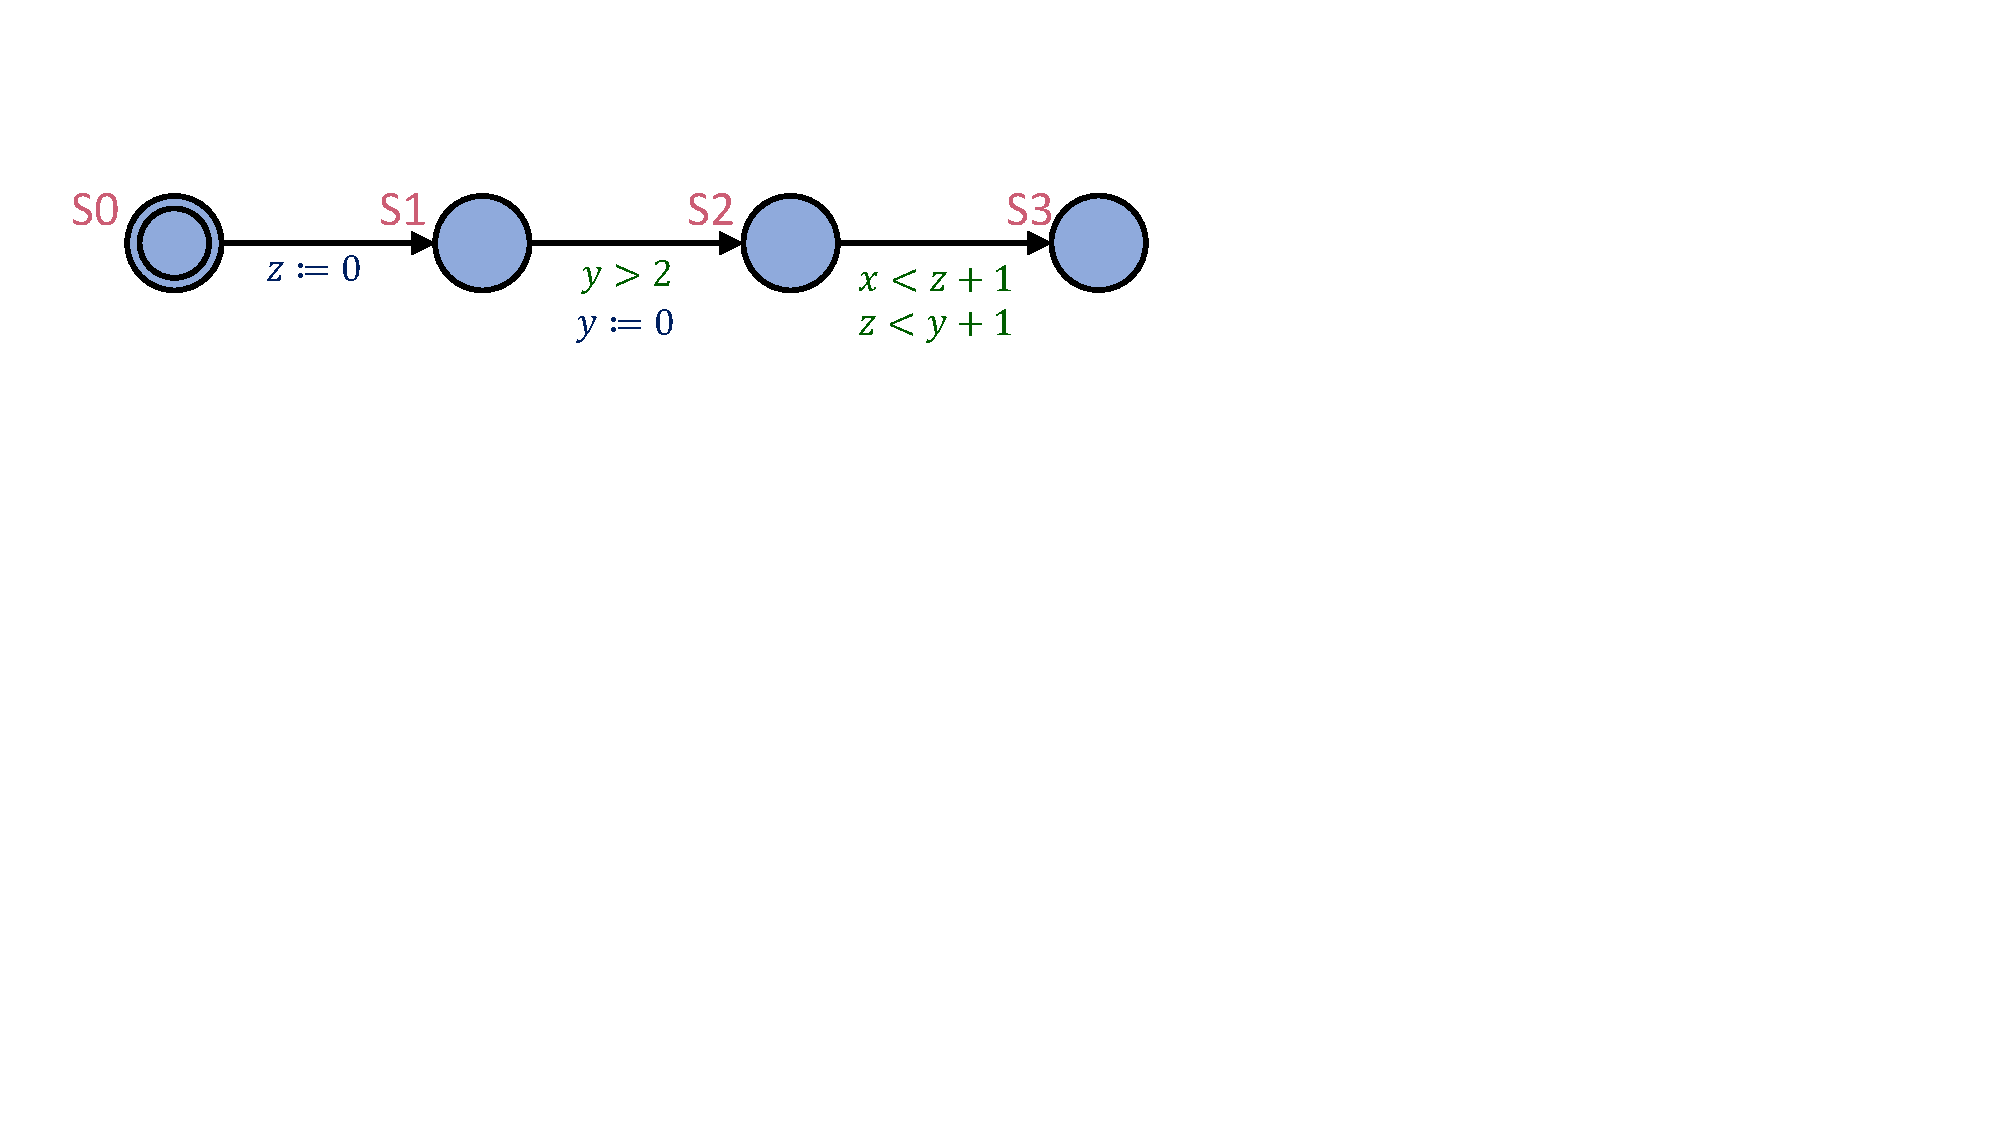
\includegraphics[width=.7\textwidth]{include/figures/splitexample_aut}
	\caption{Timed automaton example}
	\label{fig:splitex}
\end{figure}

\begin{example}


For ease of understanding the algorithm is demonstrated on the automaton in Figure \ref{fig:splitex}. The inital state is  $\langle S0, z_0 \rangle$ where $z_0$ is a zone containing only the initial valuation $v_0 \equiv 0$. The initial node is  $\langle start, z_0^\uparrow  \rangle$, where $z_0^\uparrow$ contains all states reachable form the initial state by delay. Since as time passes, the values of the three clocks will be incremented by the same value, $x$, $y$ and $z$ has the same value in each valuation contained by $z_0^\uparrow$. Since there is no invariant in location $S0$ the clocks can take any positive value. Because of this $z_0$ can be defined by the constraint $x=y=z$ (that is, $x-y = 0 \wedge y-z=0 $), and the initial node can be defined as $\langle S0; x=y=z  \rangle$.

There is only one outgoing transition from the initial location and that resets $z$, resulting in the zone defined by $x=y \wedge z=0$, which transforms into $z \leq x=y$ when delay is applied. This means the next node of the graph can be defined as $\langle S1, z \leq x=y \rangle$. There is only one outgoing transition from the location $S1$ and it has guard $y>2$. This means the transition is only enabled in the subzone $z \leq x=y>2$ (that is $z \leq x \wedge x=y \wedge y>2$). Th transition resets $y$ resulting in the zone $y=0 \wedge z \leq x > 2$. Delay can be applied and the next node of the graph turns out to be $\langle S2, z \leq x \wedge y \leq z \wedge x-y>2 \rangle$.

There outgoing transition from location $S2$ has a guard $x<z+1 \wedge z<y+1$ from which $x<y+2$ can be derived contradicting the atomic constraint $x-y>2$ in the reachable zone of location $S2$. Thus the transition is never enabled, and location $S3$ is unreachable.  

\end{example}

\begin{figure} [b]
	\centering
	\begin{minipage}[c] {0.25\linewidth}%
		%		\vspace*{1pt}%
		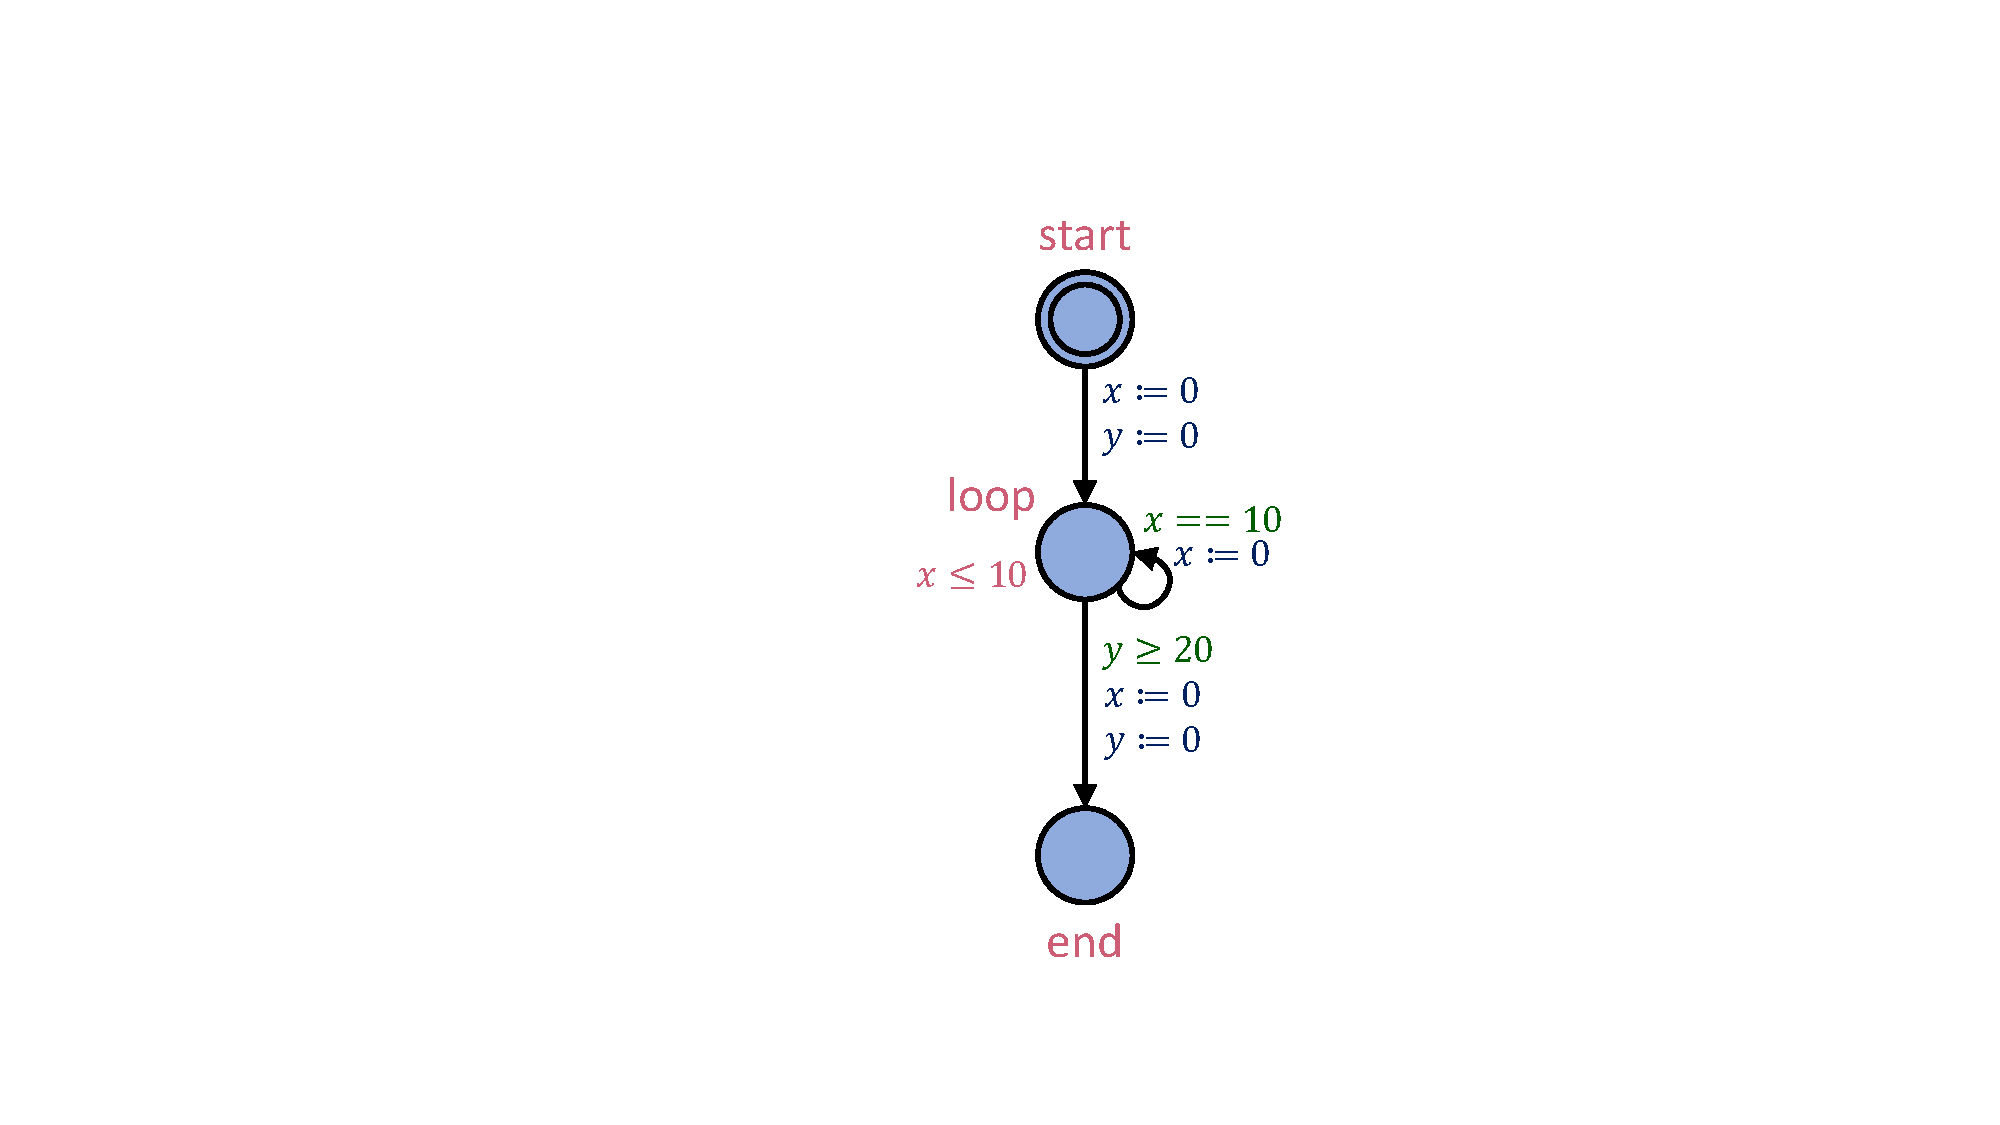
\includegraphics [width=\textwidth]{include/figures/loop_example_original}%
		%\caption{Example of a timed automaton}
	\end{minipage}%
	%	%
	\begin{minipage}[c] {0.7\linewidth}%
		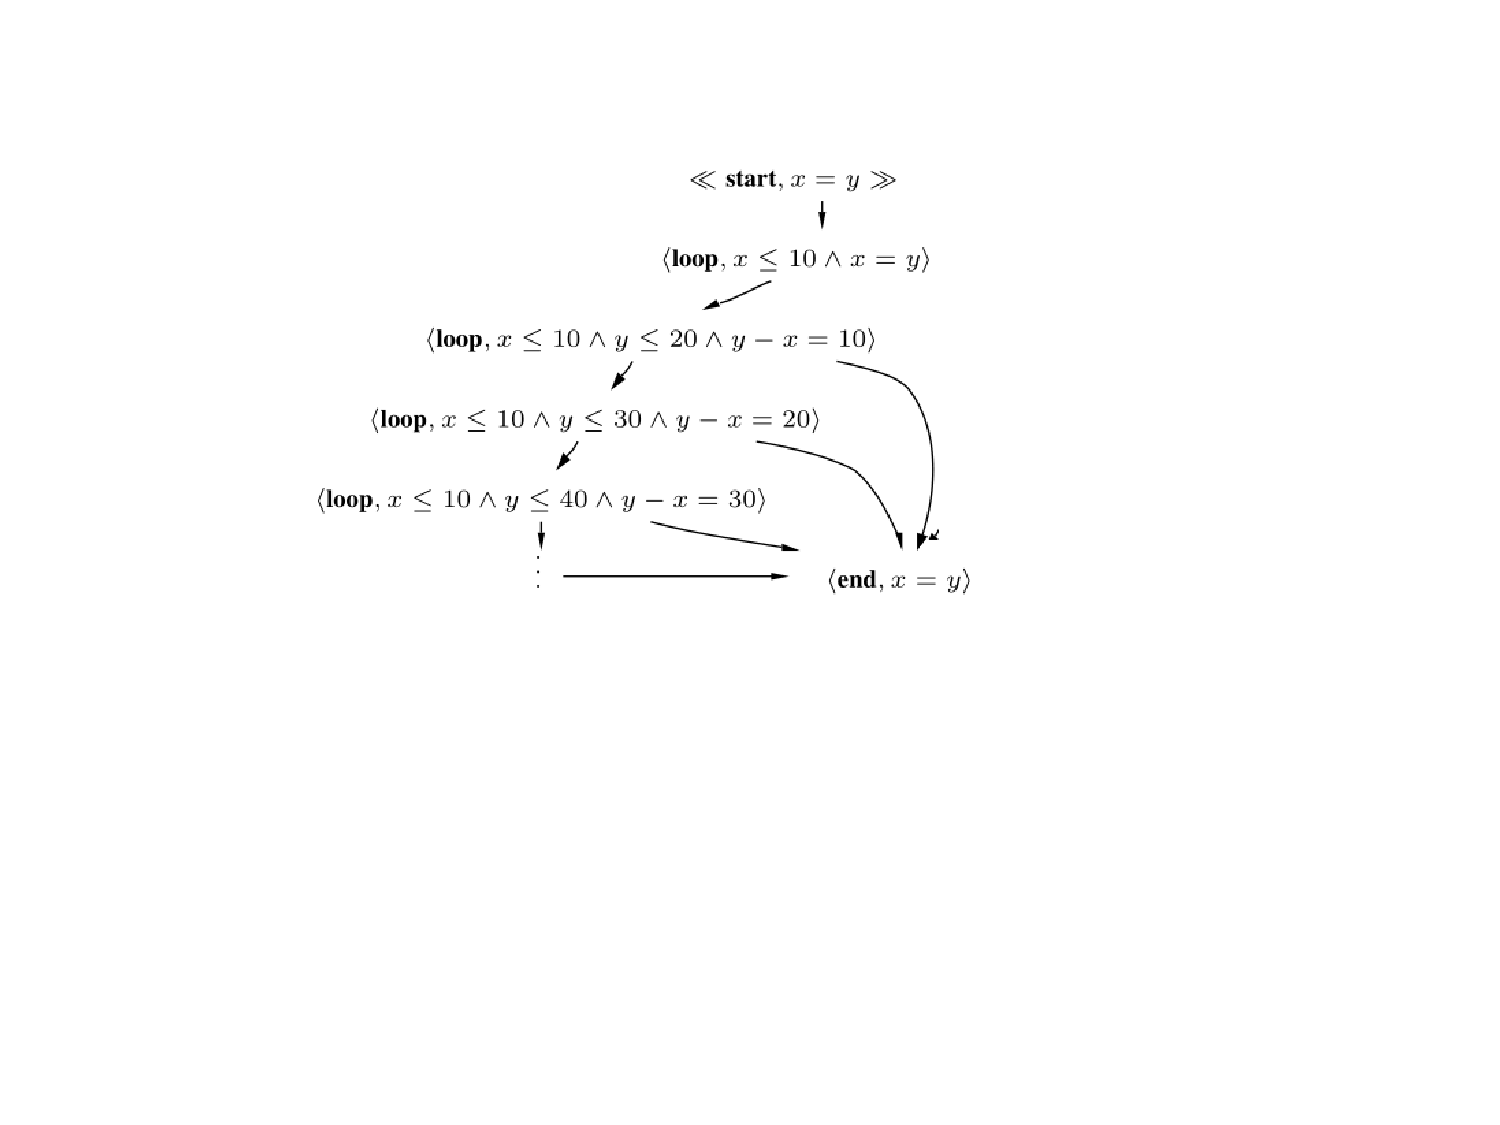
\includegraphics [width=\textwidth] {include/figures/loop_original_zonegraph}%TODO: ezt majd még vektorosítani
		%		\vspace*{4pt}%
		%		\caption{Timed automaton}
	\end{minipage}
	\caption{Timed automaton with infinite zone graph}
	\label{fig:loopinfinite}
\end{figure} 

Unfortunately, it is possible that the graph described by the previous algorithm becomes infinite. 

\begin{example}

\end{example}

Consider for example the automaton from \cite{bengtsson2004timed} in Figure \ref{fig:loopinfinite}.
Constructing the zone graph of this automaton starts similarly, with the node $\langle start, x=y \rangle$. After that both $x$ and $y$ are reset resulting in the zone defined by $x=y=0$. Location $loop$ has an invariant $x \leq 10$ that limits the applicable delay to 10, resulting in $\langle loop, x=y \leq 10 \rangle$, where only the loop-transition is enabled.

Tthe transition resets $x$ resulting in $\langle loop, x=0 \wedge y=10 \rangle$. Still only 10 units of delay is enabled, resulting in the node $\langle loop, x \leq 10 \wedge y-x=10 \rangle$.

From this node, both transitions are enabled. The loop transition increases the difference between $x$ and $y$ yielding the new node $\langle loop, x \leq 10 \wedge y \leq 30 \wedge y-x=20 \rangle$, while the other transition resets both clocks, resulting in the new node $\langle end, x=y \rangle$.

As we take the new node containing the location $loop$, and apply the loop transition over and over, a new node is always constructed with the difference growing. On the other hand, the other transition always results in $\langle end, x=y \rangle$.
Hence the (infinite) zone graph in Figure \ref{fig:loopinfinite}.

\end{example}

In order for the zone graph to be finite, a concept called \emph{normalization} is introduced in \cite{bengtsson2004timed}.

Let $k(c)$ denote the greatest value to which clock $c$ is compared in the automaton.
For any valuation $v$ such that $v(c)>k(c)$ for some $c$, each constraint in the form $c > n$ is satisfied, and each constraint in the form $c = n$ or $c < n$ is unsatisfied, thus the interval $(k(c),\infty)$ can be used as one abstract value for $c$. 

Normalization is performed on $z^\uparrow$ (before inclusion is checked) in two steps. The first step is removing all constraints of the form $x < m, x \leq m, x-y <m, x-y\leq m$ where $m>k(x)$ (so that $x$ doesn't have an upper bound), and the second step is replacing constraints of the form $x > m, x \geq m, x-y >m, x-y\geq m$ where $m>k(x)$ by $x > k(x), x \geq k(x), x-y >k(x), x-y\geq k(x)$ respectively (to define the new lower bounds).

\begin{example}
In the automaton depicted in Figure \ref{fig:loopinfinite}, $k(y)=20$ (and $k(x)=10$). This means the exact value of $y$ doesn't really matter, as long as it is greater than 20 -- the automaton will behave the exact same way if it is between 30 and 40, or if it is between 40 and 50. %We can combine the zones where $y$ is greater than 20 (and the value of $x$ is the same) into the zone $ x \leq 10 \wedge y>20 \wedge y-x>20$.
If we take this into consideration when constructing the zone graph, the zone  $x \leq 10 \wedge y-x=30$ can be normalized. In this zone, $y \geq 30 > k(y)=20$, but $x \leq k(x)$. This means we only have to consider constraints bounding $y$.
Implicitely $y \leq 40$ and $y-x \leq 30$. These constraints have to be removed from the zone. Similarly, $y \geq 30$ and $y-x \geq 30$ have to be replaced by $y \geq 20$ and $y-x \geq 20$. The resulting zone is $x \leq 10 \wedge y \geq 20 \wedge y-x \geq 20$. If we replace the original zone  $x \leq 10 \wedge y-x=30$ by this zone, and continue constructing the zone graph, the resulting graph is depicted in Figure \ref{fig:looprealgraph}.

\end{example}

\begin{figure}
	\centering
	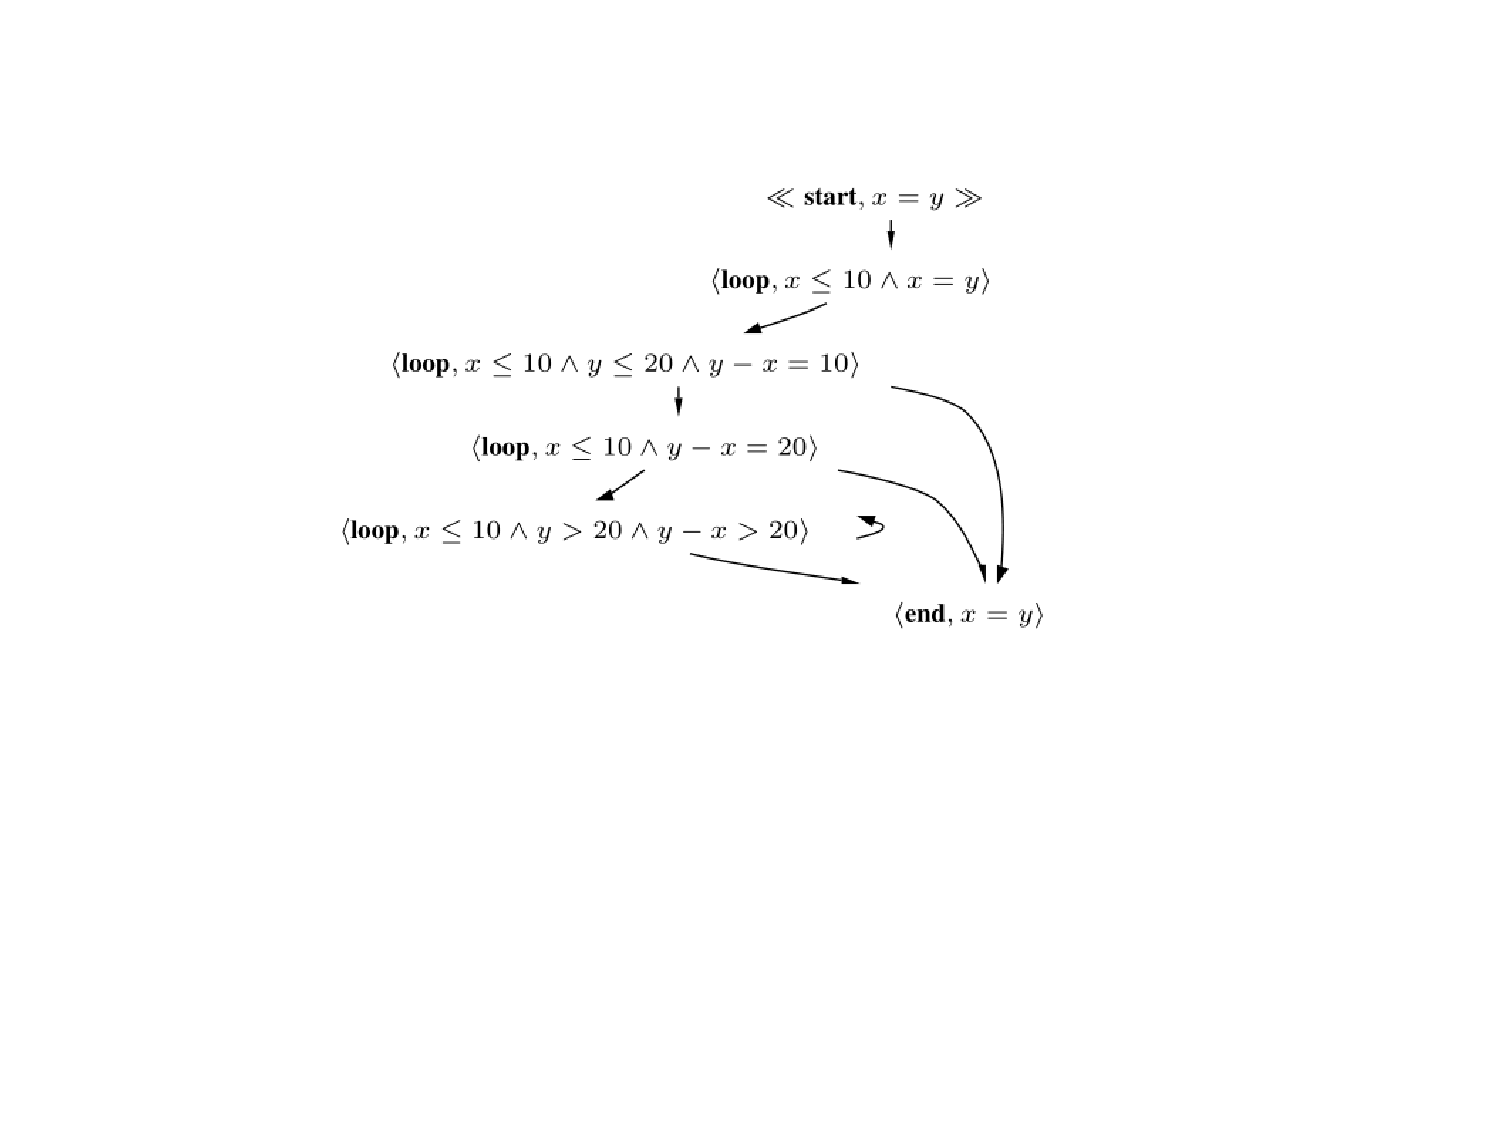
\includegraphics [width=0.7\textwidth] {include/figures/loop_real_zonegraph}%TODO: ezt majd még vektorosítani
	%		\vspace*{4pt}%
	\caption{Finite zone graph}
	\label{fig:looprealgraph}
\end{figure}

Using normalization the zone graph is finite, but unreachable states may appear in it. If the automaton doesn't have any guard or invarint of the form $c_1 - c_2 < n$, the reachability of the location in question will be answered correctly. Otherwise, the algorithm may terminate with a false positive result.

\begin{example}
	To demonstrate the incorrectness of the algorithm, consider again the automaton in Figure \ref{fig:splitex}. Recall that the reachabble states of the automaton (by our calculations) were $\langle S0,x=y=z \rangle$, $\langle S1,z \leq x=y \rangle$ and $\langle S2,z \leq y \leq z \leq y \wedge x-y > 2\rangle$ -- $S3$ is unreachable. Applying normalization leaves the states $\langle S0,x=y=z \rangle$ and $\langle S1,z \leq x=y \rangle$ unchanged, but the normalizing the reachable state in $S2$ results in $\langle S2,z \leq y \leq z \leq y \wedge x-y > 1\rangle$, where the guard can be satisfied, thus making $S3$ reachable.
\end{example}

The operation \emph{split} \cite{bengtsson2004timed} is introduced to assure correctness. Instead of
normalizing the complete zone, it is first split along the difference constraints,
then each subzone is normalized, and finally the initially satisfied constraints are reapplied to each normalized subzone. The result is a set of zones (not just one zone like before), which means multiple new nodes have to be introduced to the zone graph (all with edges representing the same transition from the original node).

\begin{example}
To demonstrate the effects of split, let us construct the zone graph of the automaton of Figure \ref{fig:splitex}. The original node remains  $\langle S0,x=y=z \rangle$, but the next node is first split along the difference constraint $x-z<1$. Instead of the node $\langle S1,z \leq x=y \rangle$, this time there are two nodes: $\langle S1, x=y \wedge x-z<1 \rangle$ and $\langle S1, x=y \wedge x-z \geq 1 \rangle$.

From  $\langle S1, x=y \wedge x-z<1 \rangle$,  $\langle S2,x-z \leq 1 \wedge z-y \leq 1\rangle$ is reachable, where the transition to location $S3$ is not enabled because of the guard $x-z < 1$.

From $\langle S1, x=y \wedge x-z \geq 1 \rangle$ the resulting zone after firing the transition is split along the constraint $z-y<1$, resulting in nodes $\langle S2, x-z \geq 1 \wedge z-y < 1\rangle$, and $\langle S2, x-z \geq 1 \wedge z-y \geq 1\rangle$. The transition to $S3$ is not enabled in either nodes. 
\end{example}

Applying split results in a zone graph, that is a correct and finite representation of the state space \cite{bengtsson2004timed}.

\subsubsection{Implementation}

Paper \cite{bengtsson2004timed} also provides an implementation of the zone domain, called \emph{Difference Bound Matrix}, or DBM for short. The idea of DBMs is based on transforming clock constraints to difference logic formulae.

Difference constraints are easy to transform as $c_1 - c_2 \geq n$ is equivalent to $c_2 - c_1 \leq -n$ (same goes for strict inequalities), and $c_1 - c_2 = n$ is equivalent to $c_1 - c_2 \geq n \bigwedge c_1 - c_2 \leq n$. In order to transform constraints of the form $x<n$ or$x \leq n$, $x \in \mathbb{C} n \in \mathds{Z}$ a new variable has to be introduced.

\begin{dfn}
	The variable denoted by $\textbf{0}$ is a special variable that has a constant value of 0. $\textbf{0}$ is not a clock variable, but can appear in clock constraints.
\end{dfn}

Using $\textbf{0}$ $x \sim n$,  $\sim \in \{\leq,<,=,>,\geq\}$ can be transformed into $x- \textbf{0} \sim n$, and all clock constraints can be transformed into the desired form. 


\begin{dfn}
	A \emph{Difference Bound Matrix} $D$ of a zone $z$ operating on $\mathcal{C}$ is a square matrix of $\abs{\mathcal{C}}+1$ rows (and columns). A row and a column is assigned to each $c \in (\mathcal{C} \cup \{\textbf{0}\})$. Each element $D_{i,j}$ of the matrix describes an upper bound on $i - j$, by storing whether the inequality is strict ($<$ or $\leq$) and the bound $n$. It is possible that there is no upper bound on $i-j$, in this case $D_{i,j}=\infty$.
	
	The DBM $D$ of zone $z$ stores all constraints bounding $z$.
\end{dfn}

%In order for operations to be effective it is required that the DBM is in a \emph{canonical} form.
%
%\begin{dfn}
%	A Difference Bound Matrix $D$ of a zone $z$ is in canonical form if for all $i,j \in (\mathcal{C} \cup \{\textbf{0}\})$, $D_{i,j}$ denotes the strictest bound on $i-j$ that can be derived from $z$.
%\end{dfn}

As zones and DBMs are different representations of the same entity, this paper uses the terms interchangably.

Many operations are defined on DBMs. The most important ones are the following:

\begin{description}
	\item [consistent($D$)] is used to decide if $D$ contains any states
	\item [relation($D$,$D'$)] tells if one of $D$ and $D'$ are contained in the other 
	\item [satisfied($D$, $m$)] wherem $m$ is a difference constraint tells if $D$ contains any states satisfying $m$ without affecting $D$
	\item [up($D$)] calcualtes $D^\uparrow$
	 \item [consistent($D$)] is used to decide if the zone represented by $D$ contains any states
	 \item [and($D$, $m$)] where $m$ is a difference constraint restricts $D$ to the states satisfying $m$
	 \item [free($D$, $c$)] where $c \in \mathcal{C}$  removes all constraints on $c$
	 \item [reset($D$, $c$,$n$)] where $c \in \mathcal{C}$, $n \in \mathds{Z}$  resets $c$ to $n$
	 \item [norm($D$, $k$)] where $k:\mathcal{C} \to \mathds{Z}$ normalizes the zone based on $k$ that assigns to each $c \in \mathcal{C}$ the highest value they are compared to in an automaton
	 \item [split($D$, $\mathcal{G}$)] where $\mathcal{G} \in \mathcal{B}(\mathcal{C})$ splits the zone based on $\mathcal{G}$ that is the set of all difference constraints appearing in an automaton.
\end{description}

\todo{egy-két mondat arról, hogy mit hogyan használunk az algoritmusban}

Implementations (pseudocodes) of these operations are provided in \cite{bengtsson2004timed}. Termination of the algorithm is also proven, but it's complexity is exponantial in the number of clocks. Because of this it is essential to reduce the number of clocks as much as it is possible, without changing the reachability property.

\subsubsection{Activity}

In \cite{RSS96*73} abstractions of the automaton are proposed to reduce the number of clock variables without affecting the operation of the automaton. The abstraction that will be used later in this paper is called \emph{activity}. A clock $c$ is considered active  at some location $l$ (denoted by $c \in Act(l)$) if its value  at the location may influence the future evolution of the system. It might be because the clock appears in the invariant of the location, or in the guard of some outgoing edges of the location, or because it is active in one of the posterior locations and its value is not reset until that location.
\begin{example}
\todo{példa}
\end{example}
The core of the algorithm for reducing the number of clock variables is to calculate $Act(l)$ for each $l \in L$, and if $Act(l)<\abs{\mathcal{C}}$ holds for each $l \in L$, the automaton can be reconstructed by \emph{renaming} variables location by location (after renaming there will be less clocks). This is true, even if all $c \in \mathcal{C}$ is active in at least one location, however, clocks might be renamed differently in distinct locations.

Before presenting how activity is calculated some new notations are introduced. Let $clk: \mathcal{B}(\mathcal{C}) \to 2^\mathcal{C}$ and assign to each clock constraints the set of clocks appear in it. Define $clk:L \to  2^\mathcal{C}$ such that $c \in clk(l)$ iff $c \in clk(I(l))$ or there exist an edge $(l,g,r,l')$ such that $c \in clk(g)$.

\emph{Activitiy} is calculated by an iterative algorithm starting from $Act_0(l)=clk(l)$ for each $l \in L$. In the $i^{th}$ iteration $Act_{i}(l)$ is derived by edtending $Act_{i-1}(l)$ by $Act_{i-1}(l')\setminus r$ for each edge $(l,g,r,l')$. The algorithm terminates when it reaches a fix point, i.e. when $Act_{i}(l)=Act_{i-1}(l)$ for each $l\in L$.

\begin{example}
	\todo{példa}
\end{example}


\subsubsection{Complexity}

As it was mentioned, reachability for timed automata without discrete variables is decidable (but it it exponential). It was also mentioned before that reachability for finite autamata extended by (discerete) variables is undecidable. Obviously, reachability of timed automata extended with discrete variables is also undecidable. However it is decidable if the value sets of the discrete variables are finite, because in this case the values can be encoded in the locations. 

\todo{módszer?}

\section{Objectives}

The goal of this paper is to provide an extendable framework for CEGAR-based algorithms deciding reachability of timed automata extended with discerete variables. Since reachability is undecidable for this type of timed automata, termination of the algorithms is not always guaranteed.

%\subsection{CEGAR}
%\subsubsection{Abstraction}
%Idea, usefulness, Times automata - zones, variables, activity, etc. +precisiont is definiálni
%\subsubsection{CEGAR-loop}
%Idea, Cegar-loop, basic cegar ideas (variable-based, statespace refinement, etc.)
%This chapter defines the important aspects of timed automata and briefly explains the reachability algorithm presented in \cite{bengtsson2004timed} and demonstrates it on some examples (based on examples, also from \cite{bengtsson2004timed}). CEGAR is also explained at a high level.


%\section{Timed Automata}

%\subsection{Reachability Analysis} \label{sec:reach}  
%
%
%
%
%
%
%%The invariant $x \leq 10$ of location $loop$ is satisfied by $z_0$, but we have to consider it when calculating the valuations reachable by delay - only the states satisfying $x \leq 10$ of $z_0^\uparrow$ are reachable. The node of the graph can be defined as $\langle loop, x=y \wedge x<10 \rangle$.
%
%%Since there is no state in $\langle loop, x=y \wedge x \leq 10 \rangle$ where $y \geq 20$ holds, the last transition will never be enabled and the zone graph is finished.
%The resulting zone graph is the following.
%
%	\[\langle S0; x=y=z  \rangle \rightarrow \langle S1, z \leq x=y \rangle \rightarrow \langle S2, z \leq x \wedge y \leq z \wedge x-y>2 \rangle \]
%
%\end{example}
%

%

%
%\begin{example}

%
%\end{example}
%	
%xxxxxxxxxxxxxxxxxxxxxxxxxxxxxxxxxxxxxxxxxxxxxxxxxxxxxxxxxxxxxxxxxxxxxxxxxxxxxxx%
%%\subsection{Implementation}
%
%\todo{Műveletekről, komplexitásról beszélni!!!}
%
%%\emph{Example:}
%%Fischer's protocol assures mutual exclusion by bounding the execution
%%times of the instructions. It can be applied to a number of processes accessing a
%%shared variable. Fig. \ref{fig:fischer}  shows the operation of a process.
%%The location \emph{critical} indicates that the process is in the critical
%%section. The value of the shared variable $id$ ranges between 0 and $n$,
%%where $n$ denotes the number of processes. The model also contains a 
%%clock variable $x_i$ for each process where $i \in \{1 \ldots n\}$ denotes the
%%identifier of the process. The constant $k$ is a parameter of the automaton.
%
%%\begin{figure}
%%	\centering
%%	\begin{minipage}[c] {0.575\linewidth}%
%%		\vspace*{1pt}%
%%		\includegraphics [width=\textwidth]{fischer_vertical}%
%%		\caption{Fischer's protocol}
%%		\label{fig:fischer}
%%	\end{minipage}%
%%	%
%%	\begin{minipage}[c] {0.425\linewidth}%
%%		\includegraphics [width=\textwidth] {fischer_product_1}%
%%		\vspace*{4pt}%
%%		\caption{Timed automaton}
%%		\label{fig:fischer_product}
%%	\end{minipage}
%%\end{figure}  
%
%%\todo{figure}
%
%%The mutual exclusion property would suggest that at any given time
%%at most one of the processes is in the \emph{critical} location. In order to
%%check the given property we must construct a timed automaton that models the
%%operation of a given number of processes.
%
%%As our definition of timed automaton only allows clock variables in the system,
%%everything else must be encoded in the location.
%%  First, to represent the
%% location of all processes simultaneously, we construct a product automaton
%% containing one location for each of the $4^n$ -- not necessarily reachable --
%% possible combinations. 
%% %For example, the initial location will be \{sleeping, sleeping, \ldots \} with
%% % an outgoing edge to each location containing a combination of $n-1$ sleeping
%% % plus one request label and the corresponding invariant. 
%% The $id$ variable can
%% be encoded in the locations the exact same way.
%% The edges, invariants, etc. should be created approriately.
%% Each location of the result automaton will be denoted by a combination of
%% the four original locations and a number representing $id$'s value. 
%%To
%%demonstrate, Fig.
%%\ref{fig:fischer_product} shows the reachable locations of the product automaton
%%of Fischer's protocol where $n=1$. The names of the locations refer to the original locations of the process, the number denotes the value of the variable $id$.
%
%
%\section{CEGAR}
%
.
%
